\subsection{Major blocks}

The flow of control begins at the bottom left of \autoref{fig:blockdiag}, with a
mic providing audio input, which is captured by MATLAB (above) and converted to
an array of integers. In ideal conditions and availability of modules, this
would be done on the arduino, with little to no performance detriment. The time
between serial inputs (based on the baud rate) is utilised to process the
incoming data into the format used through the program, which is as in the
Doobit storage system. 

\begin{figure}[ht]
    \centering
    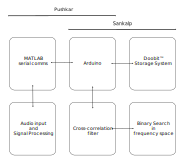
\includegraphics[height=0.4\textheight]{fig/blockdiag.pdf}
    \caption{Block diagram and work distribution.}
    \label{fig:blockdiag}
\end{figure}

After the signal has been completely read, a Dirac comb (in frequency space) is
generated from a preset range of frequencies. Ideally, a Fourier transform would
be utilized for this, but that method carries far too much resolution for just
identifying certain frequencies. A limitation that still preserves a huge space
of applications. Identification of a combination of frequencies (a trivial
extension of the current algorithm, a simple check at the end, or even better if
specific, a smaller starting set) could allow for identifying more complicated
speech patterns and more processing on subsets of the input (would be stretching
the limits of the arduino) could help in preliminary speech recognition,
possibly as a low power first gate in an always-on speech recognition system.
For example, a lower level circuit that listening for \emph{"Alexa"} and
activates a more power hungry and performant circuit for speech recognition.

To avoid processing all the frequencies, we process the entire comb at once, and
if it passes a certain threshold, we infer that one or more of the frequencies
in the comb is present in the sample. Proceeding, the comb is split halfway in
frequency space, processed depth first, to identify the frequencies present,
rejecting the entire set at any point the global maxima of its cross correlation
drops below a given threshold.

A possible optimization, abandoned in the interest of time, is to compute the
cross correlation at only a few points, utilizing optimization techniques
instead of brute forcing to find the maximum.